\chapter{Algorithmus mit Regression}

Als weitere Option die Topologie zu skalieren wurde der Algorithmus von Zacheilas et al. \cite{zacheilas_elastic_2015} für das Framework implementiert.
Er berechnet, im Gegensatz zum Algorithmus von Lohrmann et al., nicht die gegenwärtige Auslastung des Systems sondern bedient sich der Regression um den zukünftigen Zustand des Systems vorherzusagen.
Dies bedeutet konkret, dass der Algorithmus versucht präventiv auf zukünftige Ereignisse zu reagieren, während der der Algorithmus mit Warteschlangen-Theorie reaktiv agiert.
Das Ziel des Algorithmus ist die Topologie möglichst vorausschauend anzupassen.

Um den zukünftigen Zustand des Systems vorherzusagen verwenden Zacheilas et al. Gauss-Prozesse.
Gauss-Prozesse sind nicht-lineare Regressions-Verfahren und können für mehrdimensionale Regressionen verwendet werden \cite{rasmussen2004gaussian}.
Im Speziellen werden mit Hilfe des Gauss-Prozesses die verpassten Tupel eines Operators vorhergesagt.
Verpasste Tupel sind alle Tupel, die über ein Zeitfenster am Operator angefallen aber in diesem nicht abgearbeitet worden sind.
Mit Hilfe eines Gauss-Prozesses können die verpassten Tupel mit Abhängigkeit zur Zeit und zum Parallelisierungsgrad des Operators vorhergesagt werden.

Für eine vorausschauende Planung der Topologie werden Vorhersagen für mehrere in der Zukunft liegende Zeitfenster und für verschiedene Parallelisierungsgrade getroffen.
Diese werden wie in Abbildung 8.1 zu sehen in einem Graph modelliert.
Jeder Knoten \(v_{kw}\) stellt dabei eine Vorhersage für ein zukünftiges Zeitfenster \(w\) mit einem Parallelisierungsgrad \(k\) dar.
Der Operator kann zu einem gegebenen Zeitfenster einen beliebigen aber festen Parallelisierungsgrad zwischen minimalem und maximalem Parallelisierungsgrad annehmen.
Der Knoten \(v_{init}\) stellt den momentan messbaren Zustand des Operators dar.
So entsteht ein Graph der die möglichen Zustandsübergänge des Operators zu verschiedenen Zeitpunkten beschreibt.

\begin{figure}
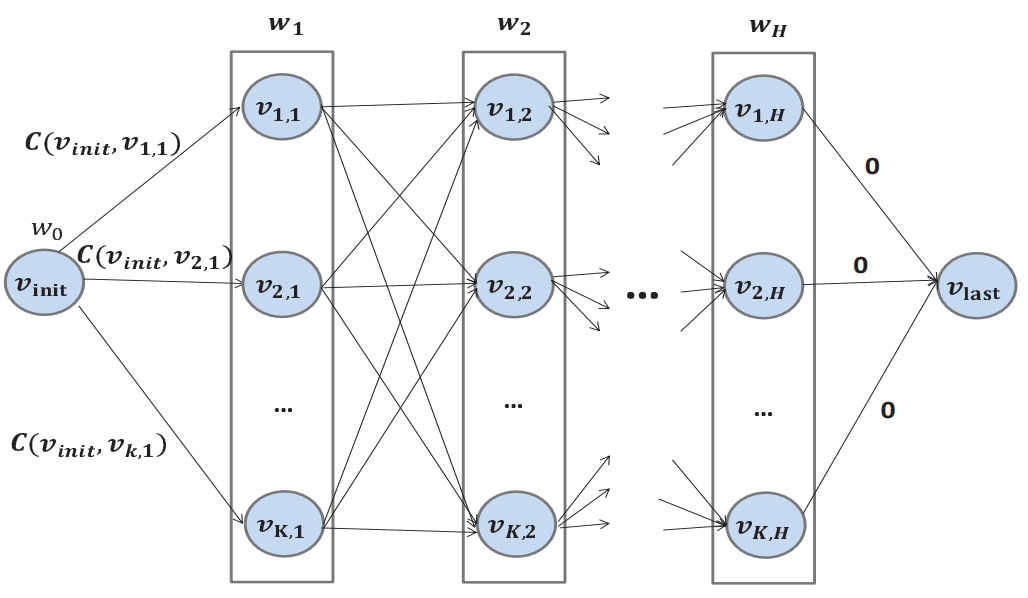
\includegraphics[scale=0.5]{ZacheilasGraph.PNG}
\caption{Graph der Zustandsübergänge \cite{zacheilas_elastic_2015}.}
\end{figure}

Um die optimalen Zustandsübergänge zu finden werden nun alle Kanten mit Gewichten versehen.
Die Gewichte der Kanten werden mit einer von Zacheilas et al. definierten Kostenfunktion bestimmt. Sie ist eine gewichtete Summe mit drei Summanden und wird durch folgenden Term definiert \cite{zacheilas_elastic_2015}:

\begin{equation*}
\begin{split}
C(v_{ij}v_{i^\prime j^\prime}) = VT_{i^\prime j^\prime} \times  C_A + p^\prime \times C_B + S(i,i^\prime) \times C_C \\
   S(i,i^\prime) =
   \begin{cases}
     0 & \text{wenn } i = i^\prime \\
     1 & \text{sonst} 
   \end{cases}
\end{split}
\end{equation*}


Der Erste der Summanden ist die Anzahl der verpassten Tupel im zukünftigen Zustand \(VT_{i^\prime j^\prime}\), die mit einem benutzerdefinierten Kostenfaktor \(C_A\) multipliziert wird.
Der zweite Summand erfasst die Kosten der Ressourcen, die benötigt werden um einen Operator auszuführen.
Die Kosten errechnen sich aus dem Produkt des zukünftigen Parallelisierungsgrades \(p^\prime\) und den benutzerdefinierten Kosten \(C_B\) eines einzelnen Tasks.
Der dritte Teil der Summe berücksichtigt den Aufwand der entsteht, wenn ein Operator skaliert wird.
Das CEP-System muss hierzu die Verarbeitung der Tupel kurzfristig stoppen und das Routing in der Topologie anpassen.
Die Kostengewichtung \(C_C\) ist ebenfalls durch den Benutzer zu bestimmen.
Sind alle Kanten gewichtet kann anschließend mittels eines Algorithmus, der den kürzesten Pfad ermittelt, die optimale Abfolge von Zustandsübergängen berechnet werden.
Der erste Zustand auf dem kürzesten Pfad durch den Graph bestimmt den Parallelisierungsgrad des Operators.

\section{Implementierung}

Im Folgenden sollen die Besonderheiten der Implementierung des Algorithmus für das Framework diskutiert werden.
Für die Implementierung des Graphen der Zustandsübergänge wurde die Bibliothek JGraphT \cite{noauthor_welcome_nodate} verwendet.
Diese liefert ebenfalls eine Umsetzung des Dijkstra-Algorithmus um den kürzesten Pfad im Graphen zu bestimmen.
Die Umsetzung der Regression mittels Gauss-Prozessen erfolgte mit der Bibliothek Smile \cite{noauthor_smile_nodate}.

\subsection{Training des Vorhersagemodells}

Die Implementierung verwendet ebenfalls das Graphen-Modell des Frameworks.
Allerdings wird für die Vorhersage eine Historie der Messdaten aus dem CEP-System benötigt.
Da das Graphen-Modell des Frameworks aber nur den aktuellen Status der Topologie repräsentiert, ist dieses nicht ausreichend.
Um das Modell für die Regression zu trainieren, werden deshalb CSV-Dateien eingelesen.
Das Regressions-Modell wird zu Beginn für alle Operatoren trainiert, sodass während des aktiven Betriebs nur noch das Graphen-Modell verwendet wird.
Während dem Betrieb können die Regressions-Modelle der einzelnen Operatoren jeweils einzeln aktualisiert werden.
Die Laufzeit eines Training-Vorgangs beträgt \(O(n^3)\) \cite{zacheilas_elastic_2015}.
Aufgrund der Laufzeit ist es sinnvoll Operatoren einzeln aktualisieren zu können während das Framework eingesetzt wird.
Bei der Aktualisierung des Modells eines Operators wird das alte Modell verworfen und durch ein neues ersetzt.
Das neue Regressions-Modell wird ausschließlich aus den zuletzt eingelesenen CSV-Daten erzeugt.

Außerdem werden in der momentan implementierten Version des Algorithmus andere Eingabewerte als in der Originalversion verwendet.
Ursprünglich werden der momentane Zeitstempel, die Tageszeit und der Wochentag für die Vorhersage der eingehenden Tupel verwendet.
Um die ausgehenden Tupel vorherzusagen wird zusätzlich der Parallelisierungsgrad des Operators verwendet.
Da die Evaluation für Zeiträume in der Größenordnung weniger Stunden vorgesehen ist, ist die Verwendung dieser Werte nicht sinnvoll.
Die Tageszeit und der Wochentag wurden daher entfernt und durch die Zeit ersetzt, die seit Beginn der Evaluation vergangen ist.

\subsection{Vorhersage von verpassten Tupeln}

Ein essentieller Teil des Algorithmus ist die Kostenfunktion, die auf der korrekten Vorhersage von verpassten Tupeln beruht.
Zacheilas et al. berechnen die Tupel wie folgt \cite{zacheilas_elastic_2015}:

\[\text{Verpasste Tupel} = \text{Anzahl eingehender Tupel} \times \text{Selektionsrate} - \text{Anzahl ausgegehener Tupel}\]

Die Selektionsrate stellt dabei das Verhältnis der Anzahl ausgegebener Tupel pro eingehendem Tupel dar.
Die Selektionsrate eines Operators wird als konstant angenommen.
Die Vorhersage von verpassten Tupeln basiert daher auf der Vorhersage der Anzahl eingehender Tupel und der Anzahl ausgehender Tupel.
Ausgehende Tupel werden im von den Autoren vorgestellten CEP-System aber nicht gemessen.
Sie berechnen deshalb die Anzahl der ausgehenden Tupel basierend auf der vergangenen Zeit, dem Parallelisierungsgrad, der vorhergesagten Task-Latenz und der Anzahl eingehender Tupel.
Da das in dieser Arbeit vorgestellte Framework die Anzahl ausgehender Tupel bereitstellt wird dieser Wert für die Umsetzung des Algorithmus nicht berechnet.
Stattdessen werden anstatt der Task-Latenz direkt die Anzahl ausgehender Tupel vorhergesagt.

\subsection{Kern der Gauss-Prozesse}
Für die Regression der Anzahl eingehender und ausgehender Tupel werden vom Algorithmus sogenannte Gauss-Prozesse verwendet.
Sie ermöglichen zu einem n-dimensionalen Eingabevektor \(x \in \mathbb{R}^n\) eine Schätzung des Zielwertes \(y\) zu berechnen.
Für diese Schätzung bedienen sich Gaußprozesse einer sogenannten Kovarianz-Matrix.
Die Kovarianz-Matrix wird mit einer Kovarianz-Funktion aus einem gegebenen Datensatz, den Trainingsdaten, berechnet.
Die Trainingsdaten bestehen aus mehreren n-dimensionalen Eingabevektoren \(x\) und deren zugehöriger Zielwert \(y\).
Die Kovarianz-Funktion \(k(x,x^\prime)\) bestimmt die Korrelation zwischen zwei Eingabevektoren \(x \in \mathbb{R}^n\) aus den Trainingsdaten.
Die Wahl der Kovarianz-Funktion hat dabei maßgeblichen Einfluss auf die berechnete Korrelation der Werte und somit auch auf das Modell des Gauss-Prozesses.
Eine Kovarianz-Funktion muss per Definition symmetrisch sein \cite{rasmussen2004gaussian}.
Die Symmetrie der Kovarianz-Funktion bedeutet, dass \(k(x,x^\prime) = k(x,x^\prime)\) gilt.
Im Bereich des maschinellen Lernens wird die Kovarianz-Funktion auch Kern genannt.
Somit besitzt jeder Gauss-Prozess einen symmetrischen Kern, mit dessen Hilfe die Kovarianz-Matrix für die Vorhersage berechnet wird.

Zacheilas et al. verwenden für Ihre Vorhersagemodelle folgenden Kern:

\[k(x, x^\prime) = \sigma^2 \exp{\left( - \frac{1}{2} \sum^{n}_{d=1} \frac{x_d-x_{d}^{\prime}}{\lambda_d}\right)}\]

Wobei \(\sigma\) und \(\lambda\) Hyperparameter des Modells darstellen.
Sie werden im Kapitel 8.2, Parameter betrachtet.
Es ist offensichtlich erkennbar, dass der von den Autoren vorgeschlagene Kernel nicht symmetrisch ist.
Das Ergebnis der Subtraktion \(x_d - x^\prime_d\) kann sowohl positiv als auch negativ sein.
Somit ist der Kern keine gültige Kovarianz-Funktion.
Für die vorliegende Implementierung wurde der Kern wie folgt geändert, sodass das Ergebnis der Subtraktion als absoluter Betrag verwendet wird.


\[k(x, x^\prime) = \sigma^2 \exp{\left( - \frac{1}{2} \sum^{n}_{d=1} \frac{|x_d-x_{d}^{\prime}|}{\lambda_d}\right)}\]

Grundsätzlich ist der Kern in Smile als Java-Interface implementiert und somit durch jede beliebige Kovarianz-Funktion austauschbar.

\subsection{Pfad-Zurückweisung}

Zacheilas et al. sehen in der Originalversion des Algorithmus eine Möglichkeit vor den gefundenen kürzesten Pfad zurückzuweisen.
Die durch den Gauss-Prozesses vorhergesagten Werte unterliegen einer Normalverteilung.
Mit Hilfe der Standardabweichung und der Normalverteilung kann berechnet werden, wie wahrscheinlich es ist, dass der vorhergesagte Mittelwert eintrifft \cite{zacheilas_elastic_2015}.
Diesen Umstand nutzen die Autoren um einen gefundenen Pfad zurückzuweisen, falls der Eintritt des vorhergesagten Wertes zu unwahrscheinlich ist.
Diese Funktionalität ist in der momentanen Version der vorliegenden Implementierung im Framework nicht vorhanden.

\section{Parameter}

Dieser Abschnitt beschreibt die Parameter die es ermöglichen den Algorithmus anzupassen.
In dem Fall des Regression-Algorithmus dienen Sie hauptsächlich dazu das unterliegende Kosten- und Regressionsmodell anzupassen.
Wie bei dem Algorithmus mit Warteschlangentheorie werden die im Graphen-Modell festgelegten minimalen und maximalen Parallelisierungsgrade berücksichtigt.
Die folgenden Parameter sind als finale statische Attribute in den Klassen der Implementierung des Algorithmus zu finden.

\subsection{Trainingsdaten}

Name: INPUT\_TRAINING\_DATA\_FOLDER / OUTPUT\_TRAINING\_DATA\_FOLDER

Standardwert: NULL

Wertebereich: alphanumerisch

Gibt den Pfad zu dem Ordner mit den Dateien an, die die Trainingsdaten für die Regressionsmodelle beinhalten.
Die Daten müssen im CSV-Format bereitgestellt werden.
Dabei ist zu beachten, dass als Trennzeichen das Leerzeichen erwartet wird.
Für jedes Vorhersagemodell wird eine eigene Datei mit Daten benötigt.
Es wird somit erwartet, dass in dem angegebenen Verzeichnis zwei Dateien pro Operator vorliegen.
Eine Datei beinhaltet die Daten um das Modell für die Anzahl eingehender Tupel zu trainieren.
Die Andere stellt die Daten des Modells für die  Anzahl ausgehender Tupel bereit.
Die Datei für eingehende Tupel muss folgenden Namen besitzen: ''<Operator>\_input\_train.csv''.
Analog gilt für ausgehende Tupel ''<Operator>\_output\_train.csv''.

Die Trainingsdaten für eingehende Tupel bestehen momentan aus drei Spalten.
Als Daten für den Eingabevektor: Unix-Zeitstempel in Sekunden, Sekunden seit Start der Anwendung.
In der letzten Spalte wird die Zielvariable Anzahl eingegangener Tupel erwartet.
Die Trainingsdaten für ausgehende Tupel umfassen vier Spalten.
Eingabevektor: Unix-Zeitstempel, Sekunden seit Start der Anwendung, Parallelisierungsgrad.
Wieder in der letzten Spalte muss die Anzahl ausgehender Tupel stehen.
Die Anzahl der Spalten für eingehende und ausgehende Tupel wird über einen Enumerator gesteuert.
Dieser muss angepasst werden, falls sich die Spaltenanzahl ändert.
Ebenso muss die Dimension von \(\lambda\) mit der Dimension der Eingabewerte übereinstimmen.

\subsection{Hyperparameter}

\begin{table}[!htbp]
\centering
\caption{Hyperparamter}
\begin{tabular}{l|r|r}
\hline
\textbf{Name} & \textbf{Standardwert} & \textbf{Wertebereich} \\
SIGMA\_INPUT & 1.0 & \(x \in \mathbb{R} > 0 \) \\
LAMBDA\_INPUT & (1.0, 1.0) &  \(x \in \mathbb{R}^2 > 0 \) \\
SIGMA\_OUTPUT & 1.0 & \(x \in \mathbb{R} 0 \) \\
LAMBDA\_OUTPUT & (1.0, 1.0, 1.0) & \(x \in \mathbb{R}^3 0\) \\
\hline
\end{tabular}
\end{table}

Die Hyperparameter dienen hauptsächlich der Konfiguration des Kerns.
Sigma ist eine Größe mit der der Kernel multipliziert wird.
Der Parameter kann dazu verwendet werden die Korrelation der Eingabevektoren grundsätzlich zu verkleinern oder zu vergrößern.
\(\lambda\) wird verwendet um die Komponenten des Eingabevektors zu gewichten.
Für den verwendeten Kernel bedeutet das, dass der negative Exponent kleiner wird wenn \(\lambda\) größer wird.
Im Umkehrschluss fällt die Korrelation für diesen Wert des Eingabevektors höher aus.

Der Wert für den Zeitstempel verdient besondere Beachtung.
Da der Zeitstempel einen absoluten Zeitpunkt markiert, verändert sich die Korrelation mit jeder Anwendung des Kernels.
Hier muss das entsprechende Element in \(\lambda\) gegebenenfalls nachjustiert werden.

Um die Anzahl ausgehender Tupel möglichst korrekt vorherzusagen sollte in \(\lambda\) berücksichtigt sein, dass der Parallelisierungsgrad im Normalfall eine kleinere Größenordnung als die anderen Werte besitzt.
Daher weist der Parallelisierungsgrad tendenziell eine höhere Korrelationen als die anderen Komponenten auf.
Dieser Umstand sollte gegebenenfalls mit \(\lambda\) ausgeglichen werden.

\subsection{Kostenfunktion}

Die vorgestellte Kostenfunktion bietet drei verschiedene Kostenfaktoren, die durch den Benutzer festgelegt werden müssen.
Die Kostenfaktoren der Funktion können über den Konstruktor angegeben werden.
Bei einem parameterlosen Aufruf des Konstruktors initialisiert dieser die Funktion mit eins.

Die Kostenfunktion implementiert ein Java-Interface und wird bei der Erzeugung der Regressions-Modelle als Parameter übergeben.
Somit ist die Kostenfunktion gegen andere Varianten austauschbar.






